\documentclass[conference]{IEEEtran}
\IEEEoverridecommandlockouts
\usepackage[nocompress]{cite}
\usepackage{amsmath,amssymb,amsfonts}
\usepackage{graphicx}
\usepackage{textcomp}
\usepackage{booktabs}
\usepackage{url}

\begin{document}

\title{Where the Lake Rises: Sentinel-1 and Sentinel-2 Evidence of Shoreline and Delta Flooding at Northern Lake Tanganyika, 2017 to 2025}

\author{
\IEEEauthorblockN{Kana Am\'ed\'ee}
\IEEEauthorblockA{Independent Researcher \\
Bujumbura, Burundi \\
kanaamedee00@gmail.com \\
ORCID 0009-0009-9620-6399 \\
Code: github.com/kanaamedee11/lake-tanganyika-flooding-sentinel}
}

\maketitle

\par\noindent{\small\bfseries\itshape Abstract. }{\small\bfseries Lake Tanganyika has been reported at record levels in 2020 to 2021 and again in 2024, with flooding around Bujumbura, Gatumba and the Rusizi delta. We ask what free Sentinel imagery shows about this at the lake's northern end from 2017 to 2025, using Sentinel-1 radar and Sentinel-2 optical data in Google Earth Engine with JRC and ESA WorldCover layers as references. Lake-wide monthly water area is nearly uninformative: the two sensors differ by 22\,km$^2$ (RMSD) on a lake of about 340\,km$^2$ and are uncorrelated from month to month, a gap larger than the 9\,km$^2$ rise in persistent water that yearly radar maps show between 2019 and 2025. The change is local. A low-lying area about 2\,km south-west of Gatumba went from water in 1\% of radar passes in 2017 to 92\% in 2025 in a steady ramp. Sentinel-2 independently shows the same ramp in the same pixels (2\% of clear observations in 2019, 99\% in 2025; correlation 0.995 with the radar across years), and it persists at different radar thresholds and in both ascending and descending orbits. The connected area is 4.5\,km$^2$ in radar and 6.2\,km$^2$ in Sentinel-2; newly persistent water in the radar maps totals about 7\,km$^2$ with default settings and 4 to 10\,km$^2$ across choices of cut and period. We state the limits: no field or lake-level data, one site, and sensors that detect open water but not flooded buildings.\par}
\vspace{0.6\baselineskip}
\par\noindent{\small\bfseries\itshape Keywords. }{\small\bfseries Lake Tanganyika, flood mapping, Sentinel-1, Sentinel-2, surface water, Rusizi delta, Burundi\par}

\section{Introduction}

Lake Tanganyika is the second deepest lake in the world and the water source and livelihood base for millions of people in four countries. In the last few years its level has risen sharply. A published water-balance study reports a significant rise between 2019 and 2020 that led to flooding, with floods in 2020 and 2021 \cite{gbetkom2024tanganyika}; press reports describe about 8{,}000 families affected around Bujumbura in April 2021 with the lake at 776.45\,m \cite{africanews2021floods}, and a record 777.2\,m in April 2024 that surpassed the 1964 maximum, with Gatumba, at the mouth of the Rusizi River, among the worst hit \cite{manishatse2024record}. The French space agency also reports that in February 2024 levels already exceeded the 2019 to 2020 maxima \cite{cnes2024lakes}. For a country with limited field monitoring, free satellite data are an obvious way to follow such events.

Two questions follow, and this paper addresses both. First, how well do the usual free sources agree on where and how much water there is at the lake's northern end? Second, where has the water actually moved? We use Sentinel-1 C-band radar \cite{torres2012s1}, which sees through cloud, and Sentinel-2 optical imagery with a water index \cite{xu2006mndwi}, which does not, processed in Google Earth Engine \cite{gorelick2017gee}, and compare them with the JRC Global Surface Water record \cite{pekel2016gsw}.

Gbetkom et al.\ \cite{gbetkom2024tanganyika} have already mapped flooding with Sentinel-2 water indices over 2017 to 2022 and related it to basin water storage. We do not repeat that work. We extend the record to 2025, add radar, compare the sensors against each other, and report in some detail what the data cannot tell us. The contributions are:
\begin{enumerate}
\item \textbf{A negative result about aggregate area.} Lake-wide monthly water area, the number most often reported, is dominated by measurement noise at this site: sensor disagreement exceeds the signal (Section~\ref{sec:agree}).
\item \textbf{A pixel-level view that finds the change.} Yearly water-frequency maps locate a progressive inundation south-west of Gatumba and show its time course (Section~\ref{sec:local}).
\item \textbf{Robustness checks.} A second sensor, three radar thresholds, an orbit-direction split, a western extension of the box, and open-lake pixels as a control for sensor drift (Section~\ref{sec:robust}).
\item \textbf{A reproducible pipeline.} One Earth Engine script and one analysis script reproduce every number and figure.
\end{enumerate}
The study has no field data and no lake-level series. It shows where the satellite record changes; it does not by itself prove why.

\section{Data and Methods}

\subsection{Study area}
The study box spans 29.20 to 29.55$^\circ$E and 3.55 to 3.15$^\circ$S (Fig.~\ref{fig:area}), about 1{,}720\,km$^2$, and contains the north-eastern end of the lake, the city of Bujumbura, the delta of the Rusizi River and the low plain around Gatumba, with steep hills to the east. A second export extends the western edge to 29.00$^\circ$E to check that nothing is cut off.

\begin{figure}[t]
\centering
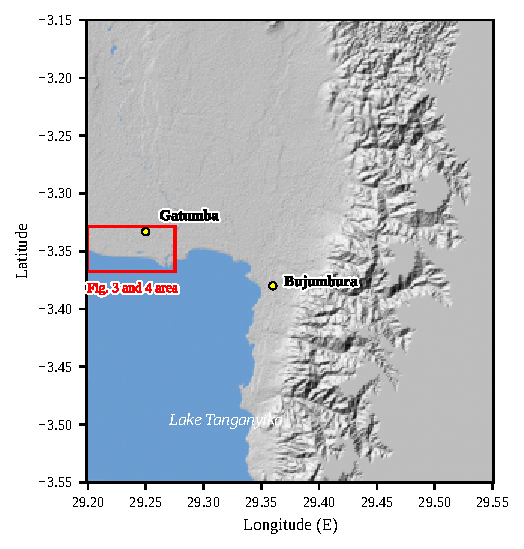
\includegraphics[width=0.78\columnwidth]{figures/fig_area.pdf}
\caption{Study box. Grey: hillshade from SRTM. Blue: JRC permanent water (occurrence of at least 50\%). The red box marks the area shown in Figs.~\ref{fig:delta} and~\ref{fig:gain}.}
\label{fig:area}
\end{figure}

\subsection{Data}
Table~\ref{tab:data} lists the sources. All are open. Processing is done in Earth Engine and only small summary files were downloaded: a monthly table and six 30\,m rasters in two exports.

\begin{table}[t]
\centering
\caption{Data sources.}
\label{tab:data}
\small
\begin{tabular}{p{1.9cm}p{5.6cm}}
\toprule
Source & Use \\
\midrule
Sentinel-1 GRD, VV & Monthly median backscatter; water if below $-16$\,dB; hill slopes ($\ge5^\circ$) excluded \\
Sentinel-2 SR, SCL & Monthly median MNDWI on clear pixels (vegetation, bare, water classes); water if above 0 \\
JRC monthly history v1.4 & Reference monthly water, valid to 2021 \\
JRC occurrence & Long-term water frequency, reference for permanent water \\
ESA WorldCover 2021 & Land cover of gained water \cite{zanaga2022worldcover} \\
Second export & Sentinel-2 yearly maps; radar at $-14$ and $-18$\,dB; radar by orbit direction; box extended west to 29.00$^\circ$E \\
SRTM & Elevation and slope \cite{farr2007srtm} \\
\bottomrule
\end{tabular}
\end{table}

\subsection{Outputs}
\textbf{Monthly series.} For each of the 108 months from January 2017 to December 2025 we compute the water area (km$^2$) in the box from each source. Sentinel-2 and JRC values are used only for months with at least 1{,}500\,km$^2$ of clear pixels (about 87\% of the box): 67 and 34 months respectively, 20 of them in both.

\textbf{Yearly frequency maps.} For each year, each Sentinel-1 scene is classified as water or not at every pixel and the share of scenes classed as water is stored as a 0 to 100 value. A pixel is \emph{persistent water} in a year if this frequency is at least 50\%. Hillside pixels are excluded (46.7\% of the box), which is why Figs.~\ref{fig:delta} and~\ref{fig:gain} show grey only where data are missing.

\textbf{Second export.} For the checks in Section~\ref{sec:robust} we also export (i) a Sentinel-2 yearly frequency map, the share of clear observations classed as water, masked where a pixel has fewer than 3 clear observations in a year; (ii) the radar frequency maps at $-14$ and $-18$\,dB; (iii) the radar frequency maps for ascending and descending passes separately; and (iv) radar and Sentinel-2 maps for a box extended west to 29.00$^\circ$E, 3.45 to 3.25$^\circ$S.

\subsection{Analyses}
\textbf{Agreement.} For pairs of sources we report the number of common months, mean difference, root-mean-square difference (RMSD), mean absolute difference, and Pearson correlation.

\textbf{Trend.} We remove the month-of-year mean, then estimate a Theil-Sen slope \cite{sen1968slope} with a 95\% interval from a moving-block bootstrap (12-month blocks, 2{,}000 resamples), which keeps the serial dependence in the monthly series.

\textbf{Change maps.} Gained water is every pixel with mean yearly frequency below 50\% in 2017 to 2019 and at least 50\% in 2023 to 2025; lost water is the reverse. We report the area, the connected components, and the WorldCover classes of gained pixels, and we vary the frequency cut (30, 50, 70\%) and the two periods.

\textbf{Control.} Sentinel-1 frequency in open-lake pixels (JRC occurrence of at least 90\% and more than 1\,km from the shore; 266\,km$^2$) should be stable. Its year-to-year range measures how much the radar's own behaviour moves, independent of any real change.

\section{Results}

\subsection{Lake-wide monthly area is nearly uninformative}
\label{sec:agree}
Fig.~\ref{fig:series} and Table~\ref{tab:agree} show the three monthly series. Over the whole period each stays close to 340\,km$^2$ even though the lake level is reported to have risen sharply, which suggests, though we did not test it, that the steep shore makes area an insensitive indicator of level. The sensors disagree by more than the total change. In the 67 clear months the mean Sentinel-1 value is 6.1\,km$^2$ below Sentinel-2, the RMSD is 22.0\,km$^2$, and the correlation is $-0.04$: knowing one sensor's value for a month tells nothing about the other's. Against the JRC monthly record, over the 34 clear months before 2022, Sentinel-1 has an RMSD of 12.6\,km$^2$ and a correlation of 0.10. The median Sentinel-1 deficit is 5.3\,km$^2$ and in 5\% of months it exceeds 31.7\,km$^2$. The largest deficits are September 2022 (282.1 against 344.6\,km$^2$ from Sentinel-2), August 2023 (294.7 against 344.3) and June 2018 (297.3 against 339.0). These are single months in which the radar misses water that the optical sensor sees; wind roughening of the water surface is a plausible cause, but we have no wind data and did not test it.

\begin{figure*}[t]
\centering
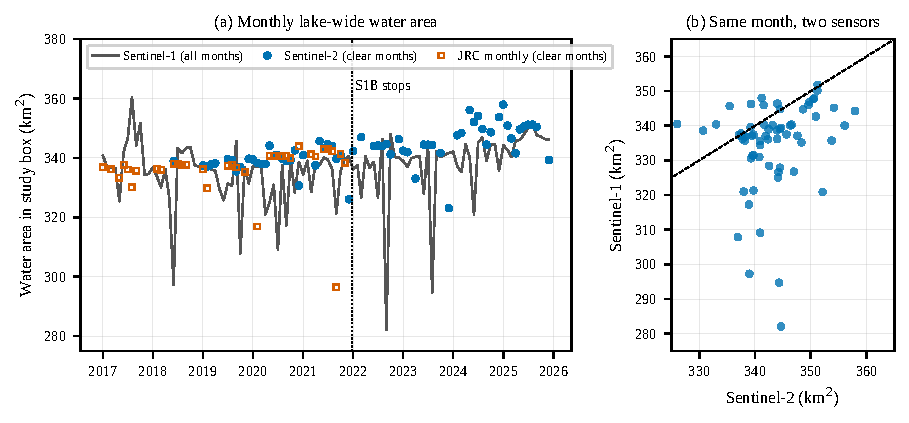
\includegraphics[width=0.92\textwidth]{figures/fig_series.pdf}
\caption{(a) Monthly water area in the study box. Sentinel-1 is shown for all months, Sentinel-2 and JRC only for months with at least 1{,}500\,km$^2$ of clear pixels. (b) Same-month Sentinel-1 against Sentinel-2.}
\label{fig:series}
\end{figure*}

\begin{table}[t]
\centering
\caption{Agreement between monthly water-area series (km$^2$). $n$: common clear months; bias: first minus second; MAD: mean absolute difference.}
\label{tab:agree}
\small
\begin{tabular}{lccccc}
\toprule
Pair & $n$ & Bias & RMSD & MAD & $r$ \\
\midrule
S1 vs S2 & 67 & $-6.1$ & 22.0 & 12.3 & $-0.04$ \\
S1 vs JRC & 34 & $-0.7$ & 12.6 & 8.8 & 0.10 \\
S2 vs JRC & 20 & $-2.6$ & 28.1 & 11.1 & 0.01 \\
\bottomrule
\end{tabular}
\end{table}

The permanent water itself is mapped well, but that is the easy part. Sentinel-1 persistent water for 2019 to 2021 overlaps the JRC long-term occurrence of at least 50\% with intersection over union 0.989 (precision 0.992, recall 0.997; 2.8\,km$^2$ extra and 1.0\,km$^2$ missed). The score is dominated by the open lake and says little about the margin. It is also not a time-matched accuracy: the JRC layer summarizes decades of imagery.

\subsection{Persistent water grows slowly}
Table~\ref{tab:annual} lists yearly values. The area of persistent water in the yearly radar maps is flat from 2017 to 2019 (338.5, 338.1, 337.9\,km$^2$) and then rises each year to 347.0\,km$^2$ in 2025, 9.1\,km$^2$ (2.7\%) above 2019. The deseasonalized monthly series give a positive slope with both sensors: $+1.1$\,km$^2$ per year for Sentinel-1 (95\% CI 0.6 to 1.6, 108 months) and $+1.8$\,km$^2$ per year for Sentinel-2 (CI 1.5 to 2.1, 67 months). The sensors agree on the sign and the order of magnitude; the point estimates differ by a factor of 1.6 and the intervals only just overlap. Both rates are small beside the monthly disagreement, which is why a trend can be found in the pooled series but individual months cannot be trusted.

\begin{table}[t]
\centering
\caption{Yearly water extent (km$^2$). Persistent: pixels classed as water in at least half of Sentinel-1 passes. Medians are of the monthly values; Sentinel-2 uses clear months only (number in brackets, shown if at least 3).}
\label{tab:annual}
\small
\begin{tabular}{lcccc}
\toprule
Year & S1 passes & Persistent & S1 median & S2 median ($n$) \\
\midrule
2017 & 112 & 338.5 & 338.8 & \\
2018 & 126 & 338.1 & 336.9 & \\
2019 & 117 & 337.9 & 333.6 & 337.8 (9) \\
2020 & 123 & 339.1 & 333.9 & 339.3 (12) \\
2021 & 136 & 340.5 & 337.6 & 340.9 (9) \\
2022 & 116 & 341.5 & 338.2 & 344.1 (8) \\
2023 & 119 & 342.2 & 340.3 & 342.2 (8) \\
2024 & 110 & 344.7 & 341.1 & 349.8 (9) \\
2025 & 151 & 347.0 & 346.3 & 350.5 (10) \\
\bottomrule
\end{tabular}
\end{table}

\subsection{The change is local}
\label{sec:local}
Pixel-level maps show where the water went. Between 2017 to 2019 and 2023 to 2025, 6.9\,km$^2$ became persistent water and 0.6\,km$^2$ ceased to be. The largest gain is a single connected area of 4.5\,km$^2$ centred at 29.234$^\circ$E, 3.348$^\circ$S, about 2\,km south-west of Gatumba, on low ground whose SRTM elevation is 772 to 778\,m (5th to 95th percentile), at the back of the shore (Figs.~\ref{fig:delta} and~\ref{fig:gain}a). Over 2017 to 2025 its mean water frequency rises from 1.2\% to 2.2, 5.7, 16.9, 34.3, 48.0, 61.5, 85.8 and 91.5\% (Fig.~\ref{fig:gain}b). The other gained pixels, 2.5\,km$^2$ in total, follow a similar ramp. The gained water lies a median 598\,m from JRC permanent water (10th to 90th percentile 60 to 1{,}587\,m).

Two points limit how this curve should be read. First, pixels were selected because their frequency was low at the start and high at the end, so the endpoints are fixed by construction; what is informative is the shape between them, a ramp over about six years rather than a step. Second, the ramp begins in 2019 to 2020 and passes 30\% in 2021, before Sentinel-1B stopped acquiring after an anomaly on 23 December 2021 \cite{esa2022s1b}, so it is not a product of that change. It lies in the same years as the reported high water of 2020 to 2021 and the record of 2024 \cite{gbetkom2024tanganyika,africanews2021floods,manishatse2024record}. Without a lake-level series we cannot test that relation quantitatively.

\begin{figure*}[t]
\centering
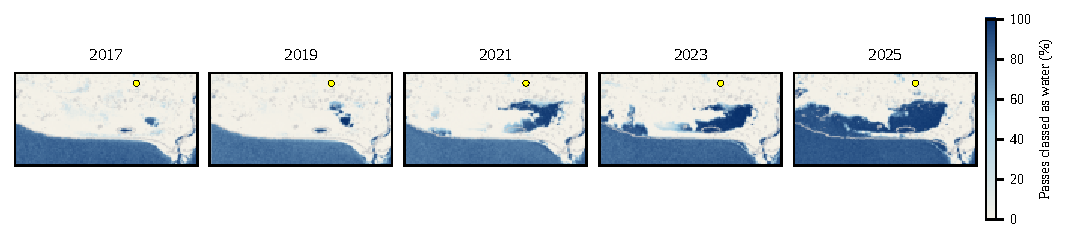
\includegraphics[width=0.96\textwidth]{figures/fig_delta_years.pdf}
\caption{Yearly Sentinel-1 water frequency in the area marked in Fig.~\ref{fig:area}. The yellow dot is Gatumba. Grey: no data (hillside mask). The open lake is at the bottom of each panel.}
\label{fig:delta}
\end{figure*}

\begin{figure*}[t]
\centering
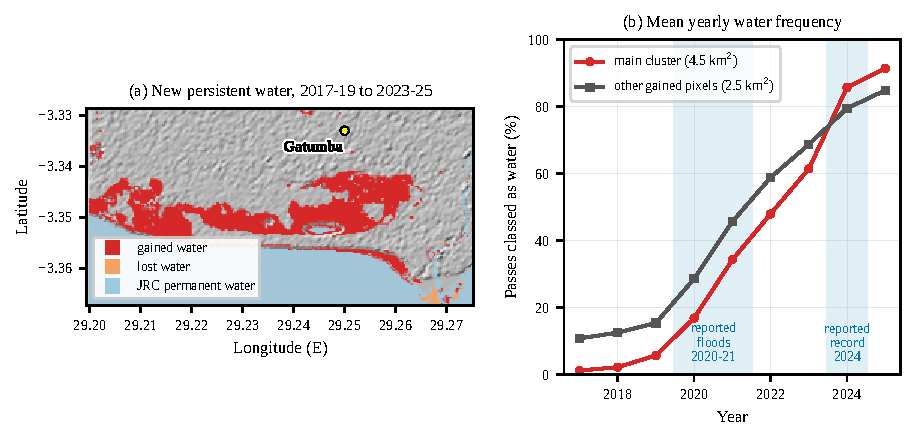
\includegraphics[width=0.96\textwidth]{figures/fig_gain.pdf}
\caption{(a) Pixels that became persistent water between 2017 to 2019 and 2023 to 2025. The map's western edge is the edge of the study box; the extended box in Section~\ref{sec:robust} shows the area is complete. (b) Mean yearly water frequency of the gained pixels. Shaded years mark reported high water, not measurements from this study.}
\label{fig:gain}
\end{figure*}

\subsection{Robustness}
\label{sec:robust}
The amount of gained water depends on analyst choices (Table~\ref{tab:sens}). Across three frequency cuts and four period pairs it ranges from 4.1 to 9.8\,km$^2$, and the single largest connected area from 1.6 to 6.4\,km$^2$. The wide spread follows from the gradual ramp: a slower or later ramp crosses a fixed cut less completely. We therefore treat the 6.9 and 4.5\,km$^2$ values as defaults, not as measurements with small error bars, and the ramp curve of Fig.~\ref{fig:gain}b as the more reliable result.

\begin{table}[t]
\centering
\caption{Gained water in km$^2$ (largest connected area in brackets) by frequency cut and comparison periods.}
\label{tab:sens}
\small
\begin{tabular}{lccc}
\toprule
Periods & Cut 30\% & Cut 50\% & Cut 70\% \\
\midrule
2017 to 2019 vs 2023 to 2025 & 8.4 (5.5) & 6.9 (4.5) & 5.6 (2.2) \\
2017 to 2018 vs 2024 to 2025 & 9.8 (6.4) & 8.3 (5.5) & 7.4 (4.6) \\
2017 to 2019 vs 2023 to 2024 & 7.0 (4.3) & 5.6 (2.4) & 5.2 (1.9) \\
2017 to 2019 vs 2022 to 2023 & 4.8 (1.8) & 4.4 (1.8) & 4.1 (1.6) \\
\bottomrule
\end{tabular}
\end{table}

\textbf{Second sensor.} Sentinel-2 sees the same pixels independently. Over the area gained in the radar maps, its yearly water frequency (share of clear observations) is 0.4\% in 2018, then 1.8, 19.8, 39.4, 50.8, 58.4, 95.5 and 98.7\% in 2019 to 2025 (Fig.~\ref{fig:checks}a). Across the eight years the radar and optical curves correlate at 0.995. The Sentinel-2 maps also give their own change map, from 2019 to 2020 against 2024 to 2025 (earlier years have too few clear observations): 10.1\,km$^2$ gained, 5.9\,km$^2$ of it one connected area, against 7.8\,km$^2$ for the radar over the same periods. 74\% of the Sentinel-2 gained pixels are also radar gained pixels (intersection over union 0.65). Sentinel-2 finds more water than the radar; flooded vegetation, whose radar return is strong, is one possible reason, but we did not test it.

\textbf{Radar threshold.} Moving the water threshold to $-14$ or $-18$\,dB keeps the ramp: the gained area's frequency rises from 5.5 to 98.0\% at $-14$\,dB and from 0.4 to 77.4\% at $-18$\,dB (Fig.~\ref{fig:checks}a), the gain is 7.6 and 7.3\,km$^2$, and its largest connected area is 4.9 and 2.6\,km$^2$. The rise in persistent water from 2019 to 2025 is 9.1\,km$^2$ at both $-14$ and $-16$\,dB. At $-18$\,dB the open lake itself is classed as water in only 51 to 66\% of passes and the persistent area in 2019 falls to 267\,km$^2$, so that threshold is too strict for this lake and we do not use it for areas.

\textbf{Orbit direction.} Splitting the radar record into ascending and descending passes shows why the open-lake control moves. In ascending passes the open lake is classed as water in 65.5 to 73.3\% of passes, in descending passes in 96.1 to 98.5\%, so the pooled 9-point drift reflects the changing mix of the two. The gained area ramps in both (ascending 1.0 to 80.9\%, descending 1.5 to 98.3\%; Fig.~\ref{fig:checks}b) with gained areas of 6.4 and 7.2\,km$^2$, so the ramp is not an artifact of orbit mix.

\textbf{Western extension.} Extending the box to 29.00$^\circ$E leaves the radar connected area at 4.50\,km$^2$ (4.46 before): it reaches only about 0.2\,km beyond the old edge and does not touch either edge of the new box, so it is not truncated. The extension adds 0.9\,km$^2$ of scattered radar gains and 1.4\,km$^2$ in Sentinel-2 west of the old edge, and the Sentinel-2 connected area is 6.2\,km$^2$, reaching about 1.7\,km west of the old edge.

\begin{figure*}[t]
\centering
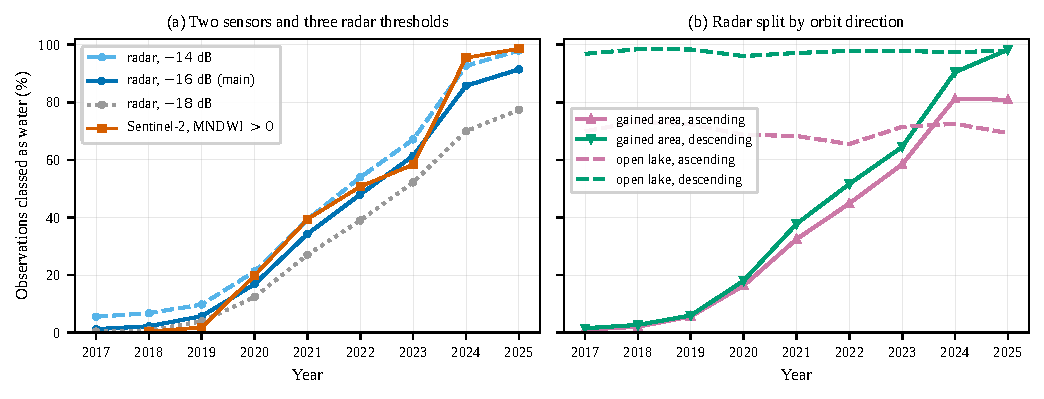
\includegraphics[width=0.92\textwidth]{figures/fig_checks.pdf}
\caption{Checks on the ramp in the gained area. (a) Radar at three thresholds and Sentinel-2. (b) Radar by orbit direction; dashed lines are the open-lake control for each direction.}
\label{fig:checks}
\end{figure*}

The pooled control shows how much the radar itself moves. Mean frequency over the open lake is 83.4, 82.9, 80.2, 77.7, 78.5, 81.0, 84.3, 84.7 and 86.9\% in 2017 to 2025, a range of 9.2 points, against the 90-point change in the gained area. The open-lake share classed as water in at least 90\% of passes is more variable, 0.2\% in 2020 and 2021 against 24.3\% in 2025. We therefore do not compare frequencies of 90\% or more across years. The orbit split above attributes much of the drift to the changing mix of ascending and descending passes (the number of passes rises to 151 in 2025 from 110 in 2024); wind and incidence angle within a direction we did not separate. Dividing the gained-area curve by the open-lake control leaves the shape unchanged (1.5 to 105\%).

Land cover in 2021 does not support an exposure estimate. Of the 6.9\,km$^2$ gained, WorldCover 2021 labels 3.5 as permanent water, 1.6 as herbaceous wetland, 1.3 as grassland, 0.5 as trees, 0.07 as cropland and 0.004 as built-up. Much of the area had therefore already turned to water or wetland by the time the map was made, so the map cannot tell us what stood there before. Radar detection of open water also cannot see flooded buildings, so the near-zero built-up figure does not mean that buildings were spared; Bujumbura's flooded streets and port were reported in the press but fall outside what these maps can show.

\section{Discussion and Limitations}

\textbf{What this adds.} The clearest finding is about method: at a site where the shore is steep and the lake is large, a lake-wide area time series carries noise larger than the signal, and a study that reports only that series could draw almost any conclusion. The change is found by looking at the margin pixel by pixel, over years instead of months. For monitoring work in Burundi this suggests reporting frequency maps and control pixels, not a single area figure.

\textbf{Limits.} (i) There are no field observations, lake-level data or very high resolution imagery, so nothing here is validated against the ground; agreement with JRC is a consistency check. (ii) The Sentinel-2 threshold (MNDWI 0) is fixed, and the radar threshold was varied only over $-14$ to $-18$\,dB. (iii) The two sensors disagree on the size of the connected area (4.5 against 6.2\,km$^2$) and we did not establish which is closer to the truth. (iv) The selection effect described in Section~\ref{sec:local} fixes the endpoints of the radar ramp; the Sentinel-2 curve is a separate measurement of the same pixels and its own change map finds the same area. (v) Within an orbit direction the open-lake control is stable, but we did not separate wind or incidence angle further. (vi) Flooded vegetation and buildings are poorly detected by either method. (vii) SRTM elevations of 772 to 778\,m are approximate in flat vegetated terrain and are not directly comparable with the reported lake levels of about 776 to 777\,m. (viii) One site, one study box. (ix) We cite press reports for events and levels; they are context, not data.

\textbf{Next steps.} The most valuable additions are a lake-level record from satellite altimetry to test the timing quantitatively, field or very high resolution observations to settle the size of the area, a method that can see flooded vegetation, and an extension to the rest of the Rusizi delta and the Burundian shore.

\section{Conclusion}

Free Sentinel data show a real, slow change at the northern end of Lake Tanganyika, but not where the usual summary number looks. Lake-wide monthly water area is swamped by sensor disagreement, while yearly water-frequency maps show a low-lying area south-west of Gatumba turning to near-permanent water in a steady ramp from 2019 to 2025. A second sensor finds the same ramp in the same pixels, and it survives different radar thresholds and both orbit directions. The size of the change depends on analysis choices and on the sensor, 4 to 10\,km$^2$ in radar, and the connected area is 4.5\,km$^2$ in radar and 6.2\,km$^2$ in Sentinel-2; its timing is consistent with reported high water, and its link to lake level remains to be tested. The work is reproducible from one Earth Engine script and one analysis script.

\bibliographystyle{IEEEtran}
\bibliography{references}

\end{document}
